\section{Fundamentals of Pressure Measurement}
The second component of the lab introduced the operation of a pressure measurement system. 
Pressure measurement is critical in chemical process industries, and engineers routinely 
work with a range of sensing technologies such as Bourdon gauges, pressure transducers, 
and differential pressure gauges. Each device is suited to different operating ranges and 
process requirements. This exercise provided hands-on exposure to these instruments as 
well as other supplementary components such as mass flow controllers, rotameters, and 
control valves.

\subsection{Objectives}
The secondary objective was to identify and characterize the components of a pneumatic 
pressure rack, including pressure gauges, transducers, flow controllers, and control valves.

\subsection{Safety}
Pressure was gradually introduced to the pressure rack to prevent system damage, with the 
pressurization rate maintained below the pressure relief valve rating of all lines. The 
system was depressurized by slowly opening the ball valves to release air, ensuring that 
pressure readings did not exceed 60 psi.

\subsection{Background}

The pressure rack system consists of four lines: one main line at the top and three 
additional lines below it.
\\[5mm]
\textbf{Main Line}

\begin{figure}
    \centering
    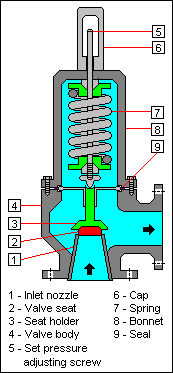
\includegraphics[width=0.2\linewidth]{figures/Pressure_Relief_Valve.png}
    \caption{Pressure relief diagram. \autocite{wikipedia_reliefvalve}}
    \label{fig:pressurereliefdiagram}
\end{figure}

The main line begins with a lockout system, which isolates the pressure source from the 
rest of the system to prevent accidental startup during maintenance. Lockout systems 
typically require multiple locks, and the system cannot be activated until all locks are 
removed.

Downstream of the lockout is a filter, which removes impurities such as water and debris 
from the air supply. When air is compressed, water vapor present in the ambient air is 
concentrated and can condense into liquid water within the system. This moisture can cause 
corrosion, degrade seals, and damage sensitive components such as valves and flow meters. 
The filter serves as the primary protection against water entering the system, reducing 
wear and erosion on system components, extending their service life and preventing failures 
such as pipe bursts or pinhole leaks.

The pressure regulator controls the pressure supplied to the rest of the system. It is 
used to incrementally adjust pressure across multiple measurements and to protect 
downstream components from hazardous pressure levels. Improper handling of this component 
could result in a system rupture.

The lubricator, positioned after the regulator, introduces small amounts of aerosolized 
oil into the airstream to reduce friction and wear on valves, gauges, and other moving 
components. The oil also helps form a seal within the system, reducing the likelihood of 
leakage and extending component lifespan.

The pressure relief valve is set to a maximum allowable pressure. When system pressure 
exceeds this threshold, the valve cap opens to release excess pressure, preventing critical 
pressure buildup that could rupture the system. The relief valve should be set to protect 
the component with the lowest pressure rating in the system. If the relief valve were set 
higher, pressure could rise to a level that exceeds the failure threshold of that component 
before the valve actuates, resulting in a rupture or catastrophic failure. The relief valve 
connects to the receiving vessel below and a ball valve to the right.

A ball valve controls flow by rotating a sphere with a through-hole along its axis. 
Aligning the hole with the flow path opens the valve; misaligning it cuts off flow. The 
state of a ball valve can be confirmed by visual inspection without instrumentation: when 
the handle is parallel to the pipe, the valve is open; when the handle is perpendicular 
to the pipe, the valve is closed. This straightforward design is widely used in industrial 
pressure systems.

\begin{figure}[H]
    \centering
    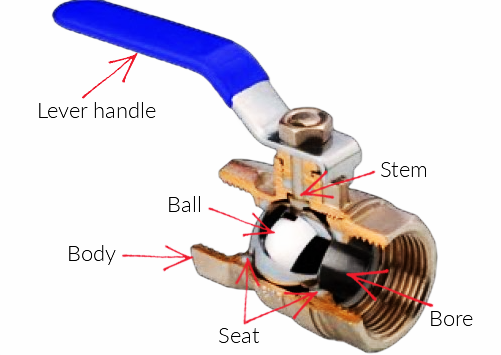
\includegraphics[width=0.5\linewidth]{figures/Ball_Valve.png}
    \caption{Ball valve diagram. \autocite{hosemaster_ballvalve}}
    \label{fig:ballvalvediagram}
\end{figure}

The receiving vessel, located directly below the pressure relief valve, stores compressed 
gas to act as a buffer, maintaining system pressure and reducing the cycle rate of the 
compressor.

Pressure in the main line is measured using a C-type Bourdon gauge, which operates on the 
principle that increased pressure causes a sealed, C-shaped tube to straighten and expand. 
This deflection is translated into a pressure reading displayed on the gauge face. The 
Bourdon gauge measures gauge pressure, which is defined relative to ambient atmospheric 
pressure rather than a perfect vacuum. Gauge pressure and absolute pressure are related by:

\begin{equation}
    P_{\text{gauge}} = P_{\text{absolute}} - P_{\text{atmospheric}}
\end{equation}

Two Bourdon gauges are present on the first line with different full-scale ranges. The 
gauge with the smaller range was used for this experiment, as the larger gauge was observed 
to read approximately half the pressure indicated by all other gauges in the system, 
suggesting it was either miscalibrated or operating well outside its accurate range. A 
gauge whose full-scale range closely brackets the operating pressures of the experiment 
produces readings with greater resolution and lower relative error than one with a much 
larger range, as an oversized scale compresses the relevant portion of the display and 
increases measurement uncertainty. Bourdon gauges remain widely used in industrial 
pressure systems. A digital gauge is also present on the first line, using internal 
components such as a strain gauge or piezoresistive sensor to measure and display pressure 
electronically.

\begin{figure}[H]
    \centering
    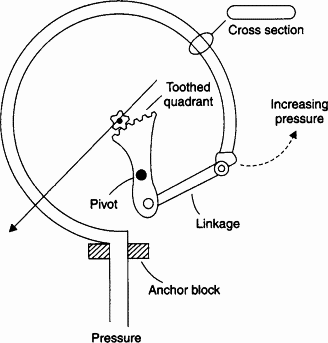
\includegraphics[width=0.3\linewidth]{figures/Bourdon_Gauge.png}
    \caption{Bourdon gauge diagram. \autocite{sciencedirect_bourdon}}
    \label{fig:bourdongaugediagram}
\end{figure}

\noindent
\textbf{Second Line}

The second line is toggled from the main line via a ball valve. It contains a mass flow 
controller (MFC), which measures and regulates gas flow using a proportional control valve 
and a closed-loop control system. The user provides an input signal, which the MFC 
compares against its internal mass flow sensor to adjust the valve accordingly. Flow rate 
is expressed as a percentage of the MFC's calibrated full-scale value.

\begin{figure}[H]
    \centering
    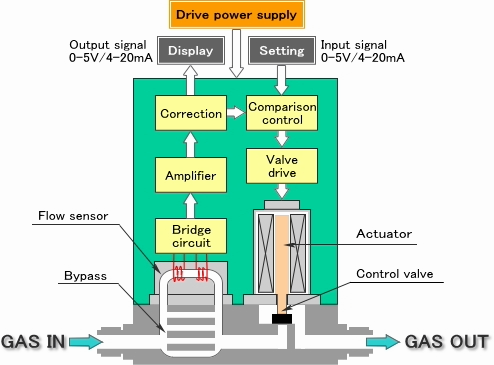
\includegraphics[scale=0.75]{figures/MFC.png}
    \caption{Mass flow controller diagram. \autocite{fcon_mfc}}
    \label{fig:massflowcontrollerdiagram}
\end{figure}

A rotameter is attached downstream of the MFC and serves as its calibration reference. 
The rotameter is a variable-area flow meter that operates by passing air through a tapered 
tube, raising a float proportionally to the flow rate. Unlike the MFC, the rotameter 
requires no power and is simple in construction.

\begin{figure}[H]
    \centering
    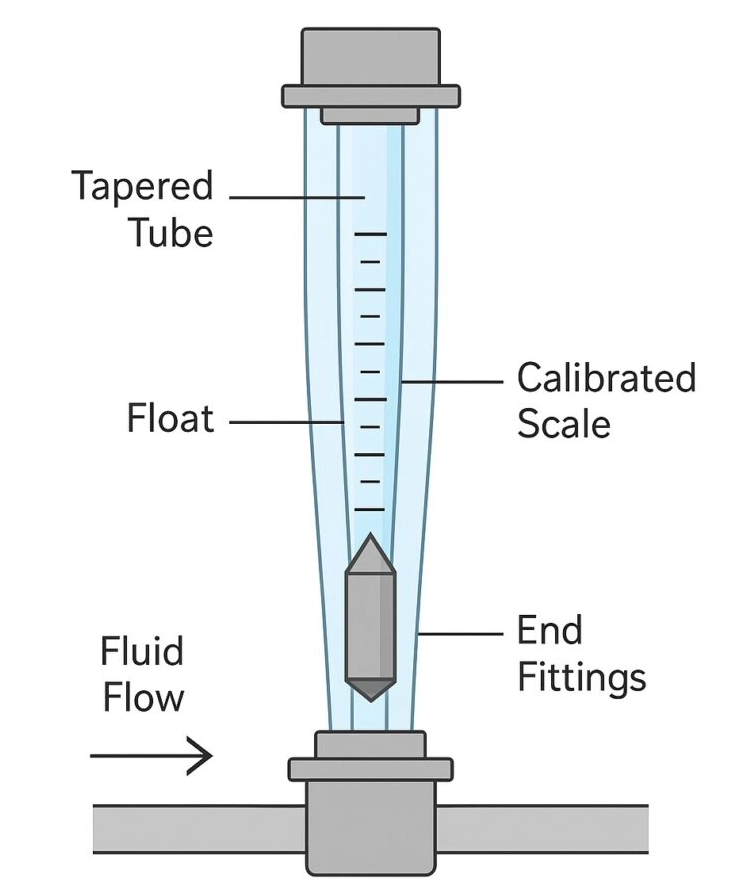
\includegraphics[scale=0.3]{figures/Rotameter.png}
    \caption{Rotameter diagram. \autocite{valuemax_rotameter}}
    \label{fig:rotameterdiagram}
\end{figure}

\noindent
\textbf{Third Line}

The third line contains a pressure transducer, which measures pressure and converts it to 
an electrical signal read and displayed by a connected computer. This type of sensor is 
common across industrial, automation, and off-road equipment applications. A Bourdon gauge 
is also present on this line, operating as described above.
\\[5mm]
\textbf{Fourth Line}

The fourth line includes a pressure regulator fixed at 15 psi, connected to an 
electro-pneumatic transducer (I/P transducer). Unlike the regulator on the main line, 
this regulator does not actively set system pressure. It is still controlled by 
the primary regulator, and this one follows accordingly. The I/P transducer converts a 
DC electrical current into a proportional pneumatic pressure signal, displayed on an 
analog dial. This pneumatic signal is used to actuate a control valve downstream, forming 
a complete electro-pneumatic control loop. As the input current to the I/P transducer is 
varied, the output pressure signal changes proportionally, which in turn adjusts the 
position of the control valve and regulates flow through the line. This arrangement is 
common in industrial process control, as it allows an electronic control system to 
manipulate pneumatic field devices without requiring direct mechanical intervention, 
enabling precise and automated flow regulation.

\subsection{Pneumatic Controls in Industrial Settings}

Pneumatic control systems are widely used in industry because they are reliable, 
cost-effective, and inherently safe in hazardous environments where electrical systems 
may pose ignition risks \autocite{dindorf_review_2025}. Compressed air is readily 
available in most industrial facilities and requires no return line, simplifying system 
design. Pneumatic actuators can generate large forces at relatively low cost, making them 
well suited for controlling valves, clamps, and other mechanical systems at scale. 
Additionally, pneumatic systems are tolerant of temperature extremes and present no 
electrical shock hazard, making them preferable in environments such as chemical plants, 
mining operations, and food processing facilities.

The U-tube manometer and Magnehelic gauge are additional pressure measurement devices 
commonly encountered in engineering practice; however, as these instruments were not 
present in the laboratory, they are not discussed further in this report.

\subsection{Methods}

The lockout system, filter, regulator, lubricator, and pressure relief valve were 
identified at the inlet of the system. The electronic components were then powered on, 
the lockout was disengaged, and the ball valves were opened slowly to establish airflow.

At the first line, the Bourdon and digital pressure gauges were identified and their 
pressure readings were recorded. At the second line, the mass flow controller and 
rotameter were identified and their readings recorded. At the third line, the Bourdon 
gauge and pressure transducer were identified and their pressures recorded. At the fourth 
line, the pressure regulator was set to 15 psi, and the I/P transducer and pneumatic valve 
were examined and their pressures recorded.

The hand regulator was then used to observe the effect of the three-way valve position on 
system pressure. With the three-way valve closed, the vessel was observed to decompress; 
with it open, system pressure was maintained. To generate the MFC calibration curve, the 
rotameter was set to flow rates of 1000, 800, 600, 400, and 200 CCM, and the corresponding 
MFC readings were recorded at each point. These values were then plotted to establish the 
relationship between the two instruments. To generate the pressure transducer calibration 
curve, system pressure was adjusted so that the Bourdon gauge read values of 40, 35, 30, 
25, and 20 psi. The corresponding transducer output was recorded at each setpoint, and 
the two datasets were plotted against each other to produce the calibration curve.

\subsection{Results}

The calibration curves for the pressure transducer and mass flow controller are presented in Figures~\ref{fig:bourdon} and~\ref{fig:rotameter}, respectively.

\begin{figure}[H]
    \centering
    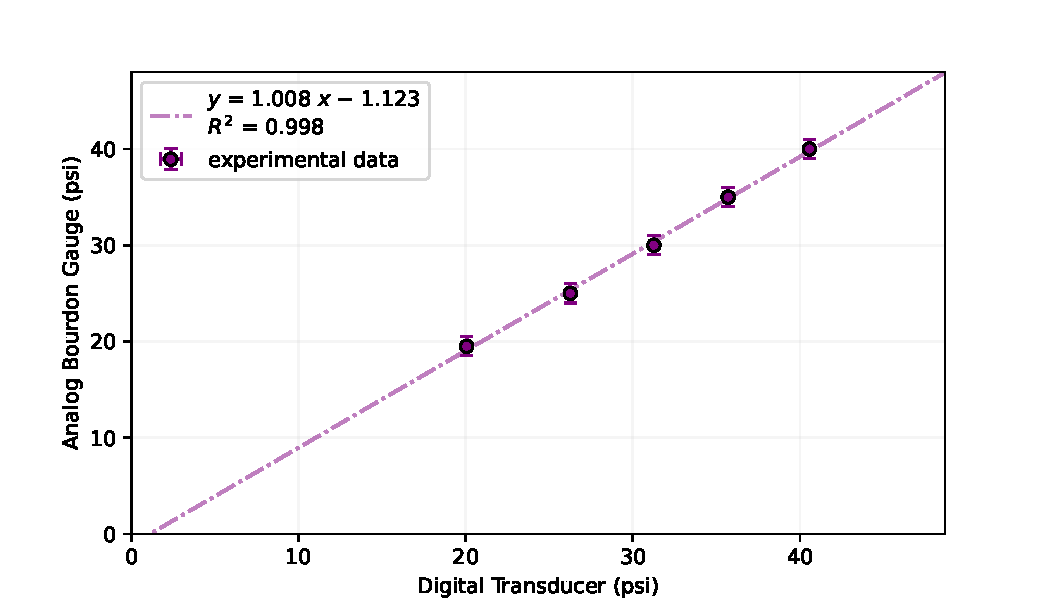
\includegraphics[width=0.8\linewidth]{figures/bourdon.pdf}
    \caption{Calibration curve for the pressure transducer. Analog Bourdon gauge pressure is plotted against digital transducer pressure. A linear fit yields $P_{\mathrm{Bourdon}} = 1.008\, P_{\mathrm{transducer}} - 1.123$ with $R^2 = 0.998$, indicating strong agreement between the two instruments.}
    \label{fig:bourdon}
\end{figure}

\begin{figure}[H]
    \centering
    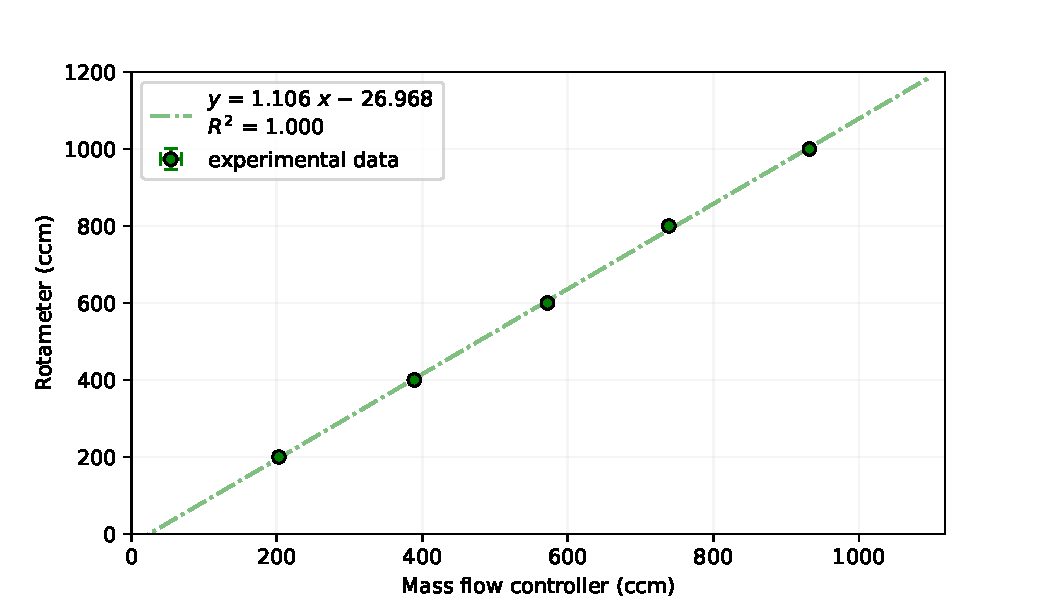
\includegraphics[width=0.8\linewidth]{figures/rotameter.pdf}
    \caption{Calibration curve for the mass flow controller. Rotameter flow rate is plotted against MFC flow rate. A linear fit yields $\dot{V}_{\mathrm{rotameter}} = 1.106\, \dot{V}_{\mathrm{MFC}} - 26.968$ with $R^2 = 1.000$, indicating an excellent linear relationship across the measured range.}
    \label{fig:rotameter}
\end{figure}

 The transducer calibration yielded a slope of approximately unity ($m = 1.008$) with a small offset ($b = -1.123$ psi) and $R^2 = 0.998$, indicating that the digital transducer and analog Bourdon gauge are in close agreement across the measured range. The small offset suggests a minor systematic difference between the two instruments, which may be attributed to Bourdon gauge resolution limitations or a slight zero-offset in the transducer. Using the linear fit, pressure may be determined from the transducer signal as:

\begin{equation}
    P_{\text{Bourdon}} = 1.008\, P_{\text{transducer}} - 1.123
\end{equation}

The MFC calibration yielded a slope of $m = 1.106$ with an offset of $b = -26.968$ ccm and $R^2 = 1.000$, indicating an essentially perfect linear relationship between the MFC and rotameter readings. The slope greater than unity suggests the MFC consistently reads slightly lower than the rotameter, which may reflect a calibration offset in the MFC relative to the reference rotameter. Using the linear fit, flow rate may be determined from the MFC signal as:

\begin{equation}
    \dot{V}_{\text{rotameter}} = 1.106\, \dot{V}_{\text{MFC}} - 26.968
\end{equation}

Calibration of these instruments is important because both the pressure transducer and MFC report electronic signals that must be related to physical quantities through a known reference. Without calibration, systematic offsets between instruments would introduce error into any measurements or process control decisions that depend on them. The strong linearity observed in both calibration curves confirms that both instruments 
are functioning correctly within the measured range and that their outputs can be reliably converted using the derived equations.